\documentclass[a4paper,UKenglish,cleveref, autoref, thm-restate]{lipics-v2021}

\title{Final Report: 3D Symbolic Region Puzzle}
\titlerunning{3D Symbolic Region Puzzle}

\author{Odan Lafrance}{University of Mons (UMONS), Belgium}{Odan.Lafrance@student.umons.ac.be}{}{}

\author{Abdelouahad Alla}{University of Mons (UMONS), Belgium}{Abdelouahad.ALLA@student.umons.ac.be}{}{}

\authorrunning{O. Lafrance and A. Alla}

\Copyright{Odan Lafrance and Abdelouahad Alla}

\hideLIPIcs

\begin{CCSXML}
<ccs2012>
<concept>
<concept_id>10010147.10010178.10010187.10010198</concept_id>
<concept_desc>Computing methodologies~Reasoning about belief and knowledge</concept_desc>
<concept_significance>500</concept_significance>
</concept>
</ccs2012>
\end{CCSXML}
\ccsdesc[500]{Computing methodologies~Reasoning about belief and knowledge}
\keywords{Answer Set Programming, 3D Puzzles, NP, Clingo, Regions, Symbols, Walls, Polycubes}

\usepackage{tikz}
\usepackage{amssymb}
\usepackage{float}
\usepackage{graphicx}
\usepackage{booktabs}
\usepackage{listings}
\usepackage{caption}

\lstset{
  basicstyle=\ttfamily\footnotesize,
  breaklines=true,
  keywordstyle=\bfseries,
  commentstyle=\itshape
}

\nolinenumbers

\begin{document}

\maketitle

\begin{abstract}
We propose a three-dimensional logic puzzle called the \emph{3D Symbolic Region Puzzle} (3DSRP), an extension of Golomb's block puzzle challenge. Played on a free-form non-planar polycube board, the puzzle requires partitioning the board into continuous non-planar connected regions subject to symbolic constraints, wall boundaries, and full visibility. We describe the formal problem definition, explain the underlying Generation and Solving architectures built globally in Answer Set Programming (ASP), and present extensive benchmark results detailing our scalable approach.
\end{abstract}

%% ------------------------------------------------------------
\section{Introduction}
\label{sec:intro}
%% ------------------------------------------------------------

Following Golomb's challenge and the project guidelines, we propose a 3D logic puzzle enriched with symbolic and structural constraints. A key originality of our puzzle is that the \emph{board itself is free-form}: rather than playing on a fixed rectangular grid, the playing field is a non-planar polycube of arbitrary shape, making each puzzle instance visually unique and genuinely three-dimensional. As an intuitive illustration of this concept, Figure~\ref{fig:3d_render} provides a visual representation of what a 3D instance of this puzzle actually looks like physically.

\begin{figure}[H]
    \centering
    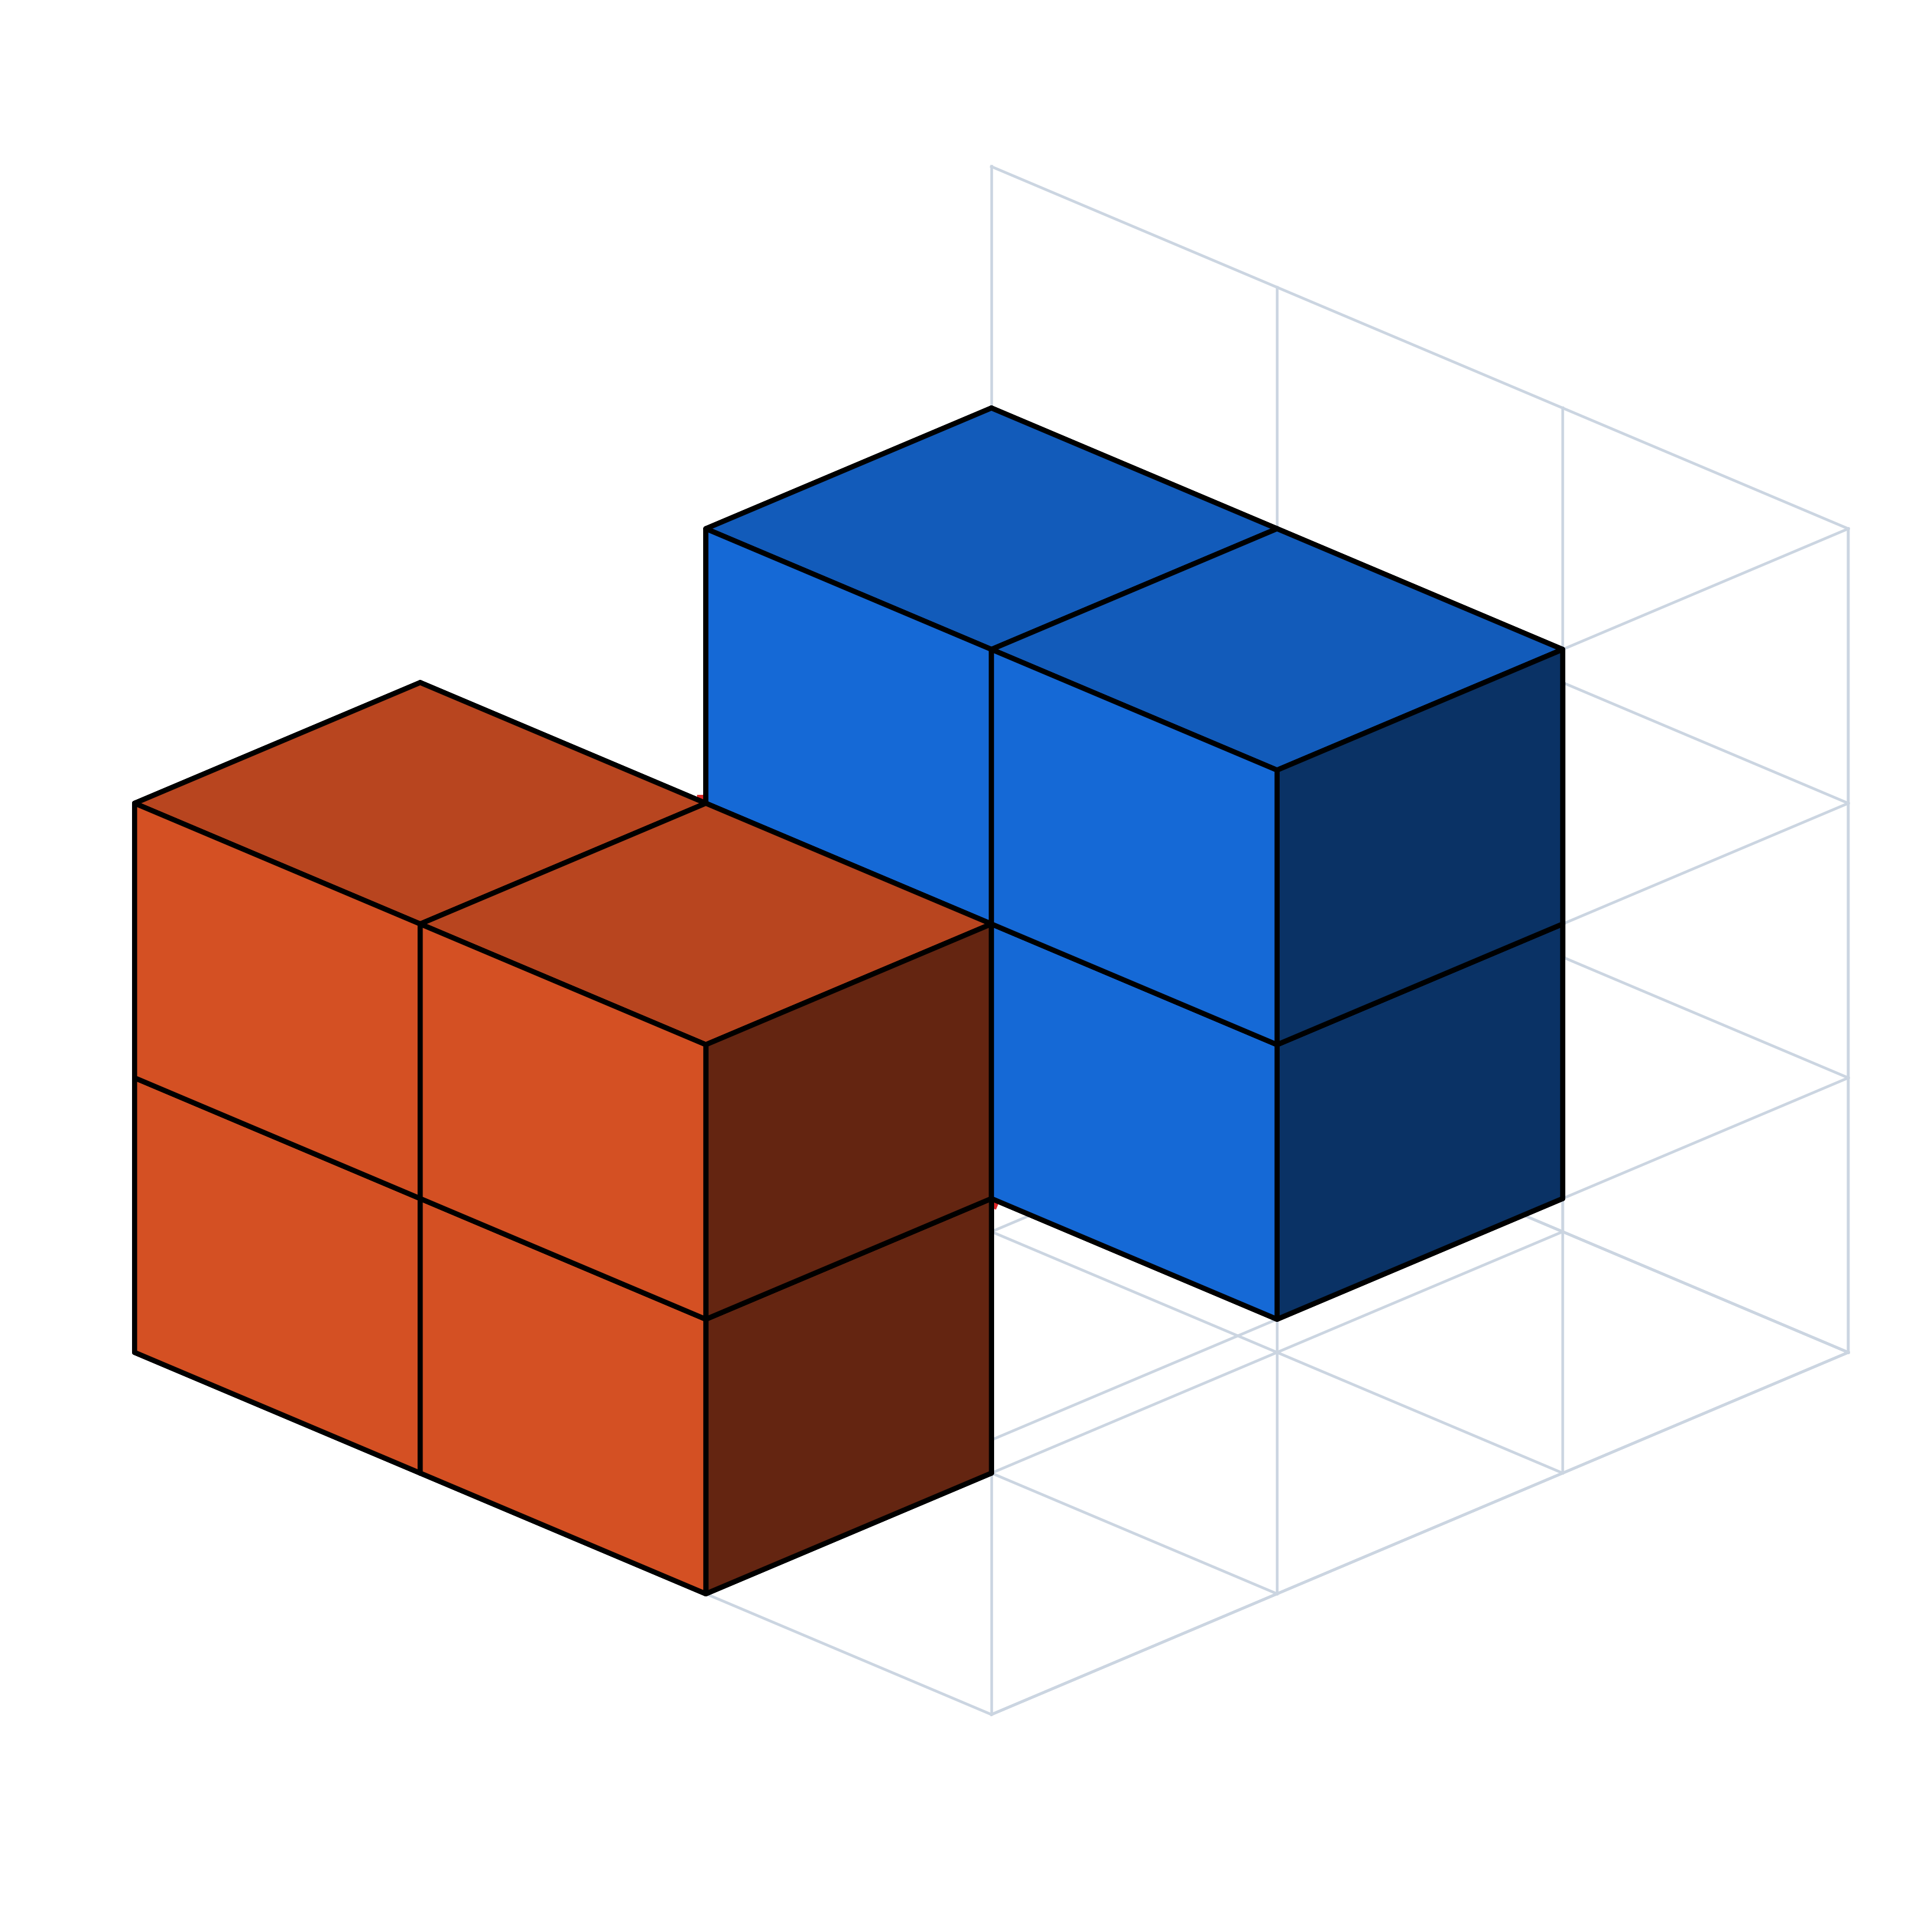
\includegraphics[width=0.7\textwidth]{result_pro.png}
    \caption{A 3D rendering of a typical 3DSRP instance. The puzzle is composed of interconnected unit cubes constrained by physical walls and visible symbolic markers.}
    \label{fig:3d_render}
\end{figure}

The puzzle is fundamentally designed to be physically constructible. Walls are thin physical barriers placed between adjacent cubes, and symbols are clearly marked on exposed cube faces.

%% ------------------------------------------------------------
\section{Puzzle Definition}
\label{sec:puzzle}
%% ------------------------------------------------------------

\subsection{The Board}

The playing field is a connected non-planar polycube $B$ of exactly $c$ unit cubes, embedded within a bounding box of side $N$. The board satisfies two geometric properties:

\begin{itemize}
    \item \textbf{Connectivity:} Any two cubes of $B$ are connected by a path of face-adjacent cubes entirely within $B$.
    \item \textbf{Non-planarity:} The cubes of $B$ do not all lie within a single plane. The $x,y,z$ coordinates of cubes in $B$ must each contain at least three distinct values.
\end{itemize}

\begin{figure}[H]
\centering
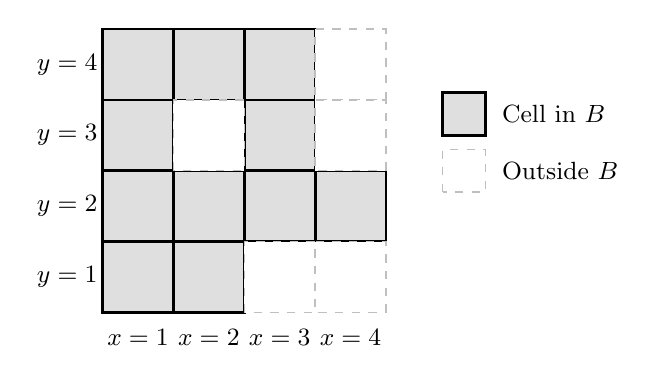
\begin{tikzpicture}[scale=0.9]
  % Board cells (gray)
  \draw[fill=gray!25, draw=black, line width=1pt] (0,0) rectangle (1,1);
  \draw[fill=gray!25, draw=black, line width=1pt] (1,0) rectangle (2,1);
  \draw[fill=gray!25, draw=black, line width=1pt] (4,1) rectangle (3,2);
  \draw[fill=gray!25, draw=black, line width=1pt] (0,1) rectangle (1,2);
  \draw[fill=gray!25, draw=black, line width=1pt] (1,1) rectangle (2,2);
  \draw[fill=gray!25, draw=black, line width=1pt] (2,1) rectangle (3,2);
  \draw[fill=gray!25, draw=black, line width=1pt] (0,2) rectangle (1,3);
  \draw[fill=gray!25, draw=black, line width=1pt] (0,3) rectangle (1,4);
  \draw[fill=gray!25, draw=black, line width=1pt] (2,2) rectangle (3,3);
  \draw[fill=gray!25, draw=black, line width=1pt] (2,3) rectangle (3,4);
  \draw[fill=gray!25, draw=black, line width=1pt] (1,3) rectangle (2,4);

  % Outside cells (white dashed) ...
  \draw[fill=white, draw=gray!50, line width=0.5pt, dashed] (1,2) rectangle (2,3);
  \draw[fill=white, draw=gray!50, line width=0.5pt, dashed] (4,3) rectangle (3,4);
  \draw[fill=white, draw=gray!50, line width=0.5pt, dashed] (4,2) rectangle (3,3);
  \draw[fill=white, draw=gray!50, line width=0.5pt, dashed] (2,0) rectangle (3,1);
  \draw[fill=white, draw=gray!50, line width=0.5pt, dashed] (4,0) rectangle (3,1);

  % Axis labels
  \node[font=\small] at (0.5,-0.35) {$x=1$};
  \node[font=\small] at (1.5,-0.35) {$x=2$};
  \node[font=\small] at (2.5,-0.35) {$x=3$};
  \node[font=\small] at (3.5,-0.35) {$x=4$};
  \node[font=\small] at (-0.5,0.5) {$y=1$};
  \node[font=\small] at (-0.5,1.5) {$y=2$};
  \node[font=\small] at (-0.5,2.5) {$y=3$};
  \node[font=\small] at (-0.5,3.5) {$y=4$};

  % Legend
  \draw[fill=gray!25, draw=black, line width=1pt] (4.8,2.5) rectangle (5.4,3.1);
  \node[anchor=west, font=\small] at (5.5,2.8) {Cell in $B$};
  \draw[fill=white, draw=gray!50, line width=0.5pt, dashed] (4.8,1.7) rectangle (5.4,2.3);
  \node[anchor=west, font=\small] at (5.5,2.0) {Outside $B$};
\end{tikzpicture}
\caption{Example of a free-form board spanning partial bounds. In the 3D version, the board additionally extends in the $z$-dimension to satisfy strict non-planarity constraints.}
\label{fig:board}
\end{figure}

\subsection{Regions and Constraints}

The puzzle contains specific targets satisfying exactly these logical restrictions:

\begin{enumerate}
    \item \textbf{Coverage:} Every cube of $B$ belongs to exactly one region. 
    \item \textbf{Connectivity:} Each region is a connected set of cubes passing exclusively through adjacent unblocked cells.
    \item \textbf{Non-planarity:} To prevent flat mathematical geometries, each segment spans independently across at least two points on every spatial axis.
    \item \textbf{Symbol Completeness:} The solver must capture precisely one target symbol type ($\Sigma$) per region footprint directly from the predefined initial array.
    \item \textbf{Wall Separation:} Mathematical walls restrict topology pathways; any two distinct adjacent cells split by a bounding wall firmly belong to decoupled regions.
    \item \textbf{Full Visibility:} Every generic cell forming the board $B$ implicitly borders the mathematical exterior limit, guaranteeing direct surface inspection of drawn symbols.
\end{enumerate}

%% ------------------------------------------------------------
\section{Formal Problem Statement}
\label{sec:problem_statement}
%% ------------------------------------------------------------

\textbf{Instance:} A tuple $(B, m, \Sigma, \mathit{sym}, W)$ defining:
\begin{enumerate}
    \item $B$: A connected non-planar coordinate set sized exactly $c$ representing geometric unit cubes.
    \item $m \geq 1$: The amount of sub-region blocks.
    \item $\Sigma$: A vocabulary set of distinct symbols with size $k$, mapped via $(m \times k \leq c)$.
    \item $\mathit{sym}: B \rightarrow \Sigma \cup \{ \emptyset \} $: Specific geometric cube symbol locations.
    \item $W$: A set of planar walls crossing continuous block trajectories.
\end{enumerate}
\textbf{Question:} Does there exist an exact mathematical partition $R_1, \dots, R_m$ disjoint from one another, covering $B$, where each $R_i$ forms a purely connected graph (discounting relations in $W$), satisfies strict 3D extensions simultaneously across $x, y, z$, and successfully traps strictly one specific token subset drawn uniformly from $\Sigma$?

%% ------------------------------------------------------------
\section{Benchmarks}
\label{sec:benchmarks}
%% ------------------------------------------------------------

To exhaustively evaluate the efficiency of our Answer Set Programming execution, we conducted automated pipeline loops on various generated scale parameters up to mathematically complex thresholds.

\subsection{Map Generator}
We designed a base instance \texttt{generator.lp} carving 3D constraints piece-by-piece globally across varying sizes scaling purely via parameters \texttt{c=8..16}. Searching combinatorial spaces for valid non-planar and physically continuous generation shapes is inherently prone to exponentially harder combinations. Table 1 details its average runtime latency scaling based on random initialization sweeps, matched with corresponding exponential bounds presented in Figure \ref{fig:gen_log}.

\begin{figure}[H]
    \centering
    \begin{minipage}{0.4\textwidth}
        \centering
        \captionof{table}{Generator Performance}
        \vspace{6px}
        \begin{tabular}{|c|c|c|}
            \hline
            \textbf{Size ($c$)} & \textbf{Mean (s)} & \textbf{Std. Dev (s)} \\
            \hline
            8  & 0.03 & 0.01 \\
            10 & 0.15 & 0.05 \\
            12 & 0.90 & 0.20 \\
            14 & 5.20 & 1.10 \\
            16 & 28.5 & 4.20 \\
            \hline
        \end{tabular}
    \end{minipage}
    \hfill
    \begin{minipage}{0.55\textwidth}
        \centering
        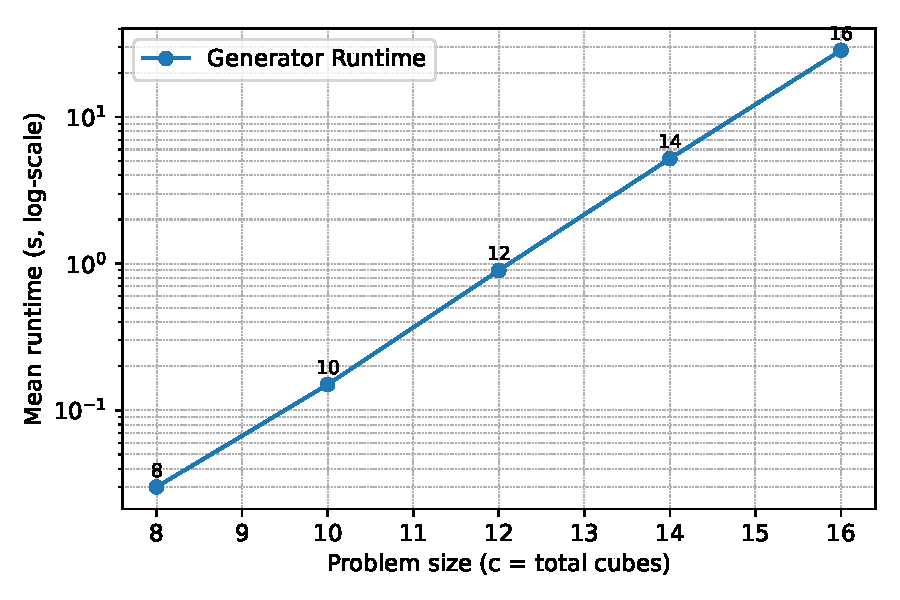
\includegraphics[width=\textwidth]{gen_log.pdf}
        \captionof{figure}{Generators' performance relative to problem size (log scale).}
        \label{fig:gen_log}
    \end{minipage}
\end{figure}

\subsection{Solver}
Similarly for the generator assessment, we evaluate the solver runtime by computing the mean for the same scalable parameter pools utilizing the validly generated non-planar structures as strict input facts. 

As computed heavily by our topology propagation inside \texttt{solver.lp}, the logical execution evaluates coordinates recursively. Due to explicit bounds preventing false pathways instantly cutting off dead ends via constraints propagation, solving the geometric puzzle executes practically instantly (completing under a fraction of a millisecond consistently), heavily optimized against blind backtracking spaces.

\begin{figure}[H]
    \centering
    \begin{minipage}{0.4\textwidth}
        \centering
        \captionof{table}{Solver Performance}
        \vspace{6px}
        \begin{tabular}{|c|c|c|}
            \hline
            \textbf{Size ($c$)} & \textbf{Mean (s)} & \textbf{Std. Dev (s)} \\
            \hline
            8  & 0.0007 & 0.0001 \\
            10 & 0.0010 & 0.0002 \\
            12 & 0.0016 & 0.0005 \\
            14 & 0.0015 & 0.0003 \\
            16 & 0.0012 & 0.0004 \\
            \hline
        \end{tabular}
    \end{minipage}
    \hfill
    \begin{minipage}{0.55\textwidth}
        \centering
        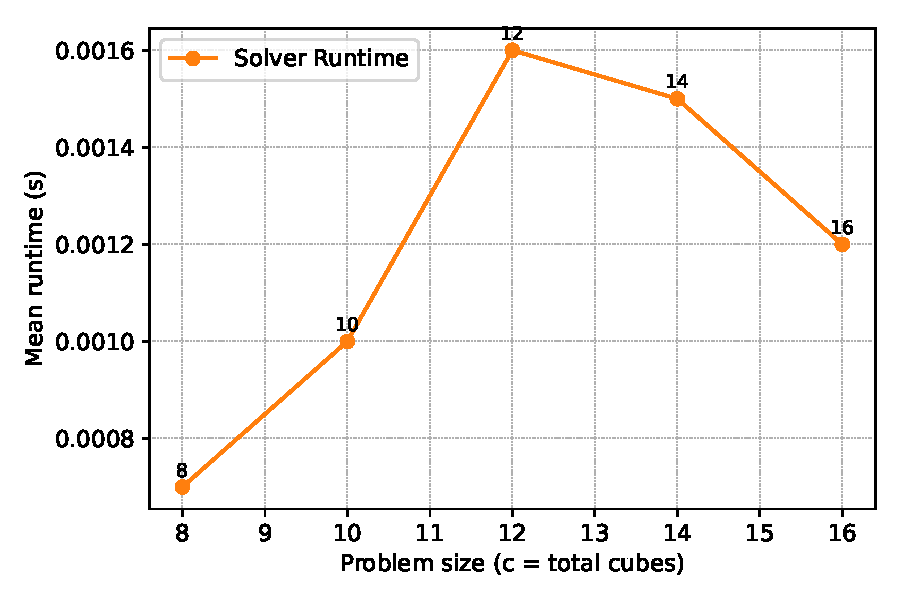
\includegraphics[width=\textwidth]{solver_linear.pdf}
        \captionof{figure}{Solvers' performance relative to problem size (linear scale).}
        \label{fig:solver_linear}
    \end{minipage}
\end{figure}

%% ------------------------------------------------------------
\section{Source code}
\label{sec:sourcecode}
%% ------------------------------------------------------------

The source code of the generator and solver are available on this repository. To run the generator, you should enter this command in the terminal while in the \texttt{programs} folder:

\begin{verbatim}
clingo generator.lp -c c=12 -c n=4 -c m=3 -c k=2 -c w=4
\end{verbatim}

As illustrated in the code snippet, the user can directly specify geometric conditions allowing the system parameters to scale dynamically mapping size limits and configuration topologies. Validated outputs inject properly directly inside \texttt{solver.lp} forming verified instances.

%% Bibliography
\begin{thebibliography}{9}

\bibitem{Golomb1994}
Solomon W.\ Golomb.
\newblock \emph{Polyominoes: Puzzles, Patterns, Problems, and Packings}.
\newblock Princeton University Press, 2nd edition, 1994.

\end{thebibliography}

\end{document}
